\section{Supplementary Human Connectome Project Results}
\label{sec:Cohen_supp_CI_figs}

%\setcounter{figure}{0}    

\begin{table}[!htbp]
\hspace*{-0.5cm}
\begin{adjustbox}{center}
\centering
    \begin{tabular}{cm{50mm}m{50mm}m{50mm}}
       \toprule
         Threshold $c$ & \hspace{1.4cm} Sagittal (X = 63) & \ \hspace{1.15cm} Coronal (Y = 130) & \hspace{1.0cm} Axial (Z = 124)\\
        \midrule
        0.5 Cohen's $d$ & 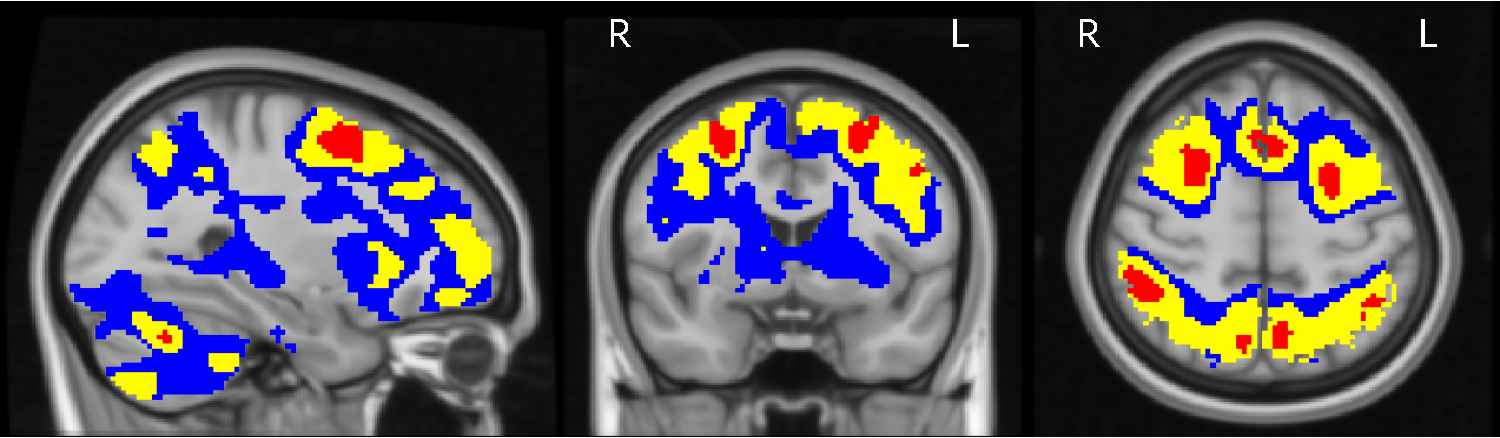
\includegraphics[height=45.5mm]{CIC_Fig1_Algorithm1_c05.pdf}\\
        0.8 Cohen's $d$ & 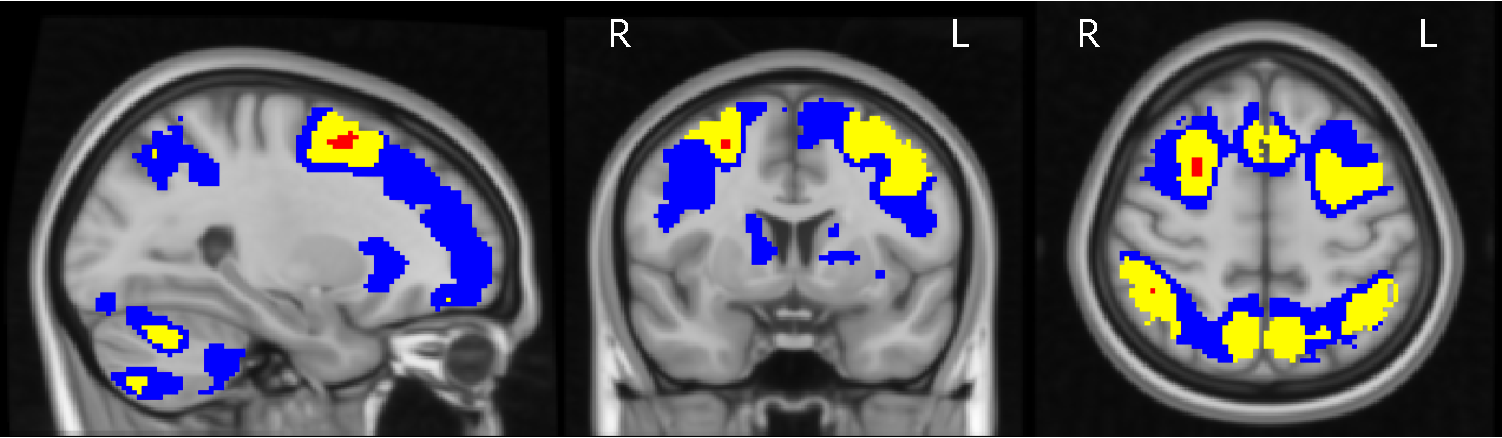
\includegraphics[height=45.5mm]{CIC_Fig1_Algorithm1_c08.pdf}\\
        1.2 Cohen's $d$ & 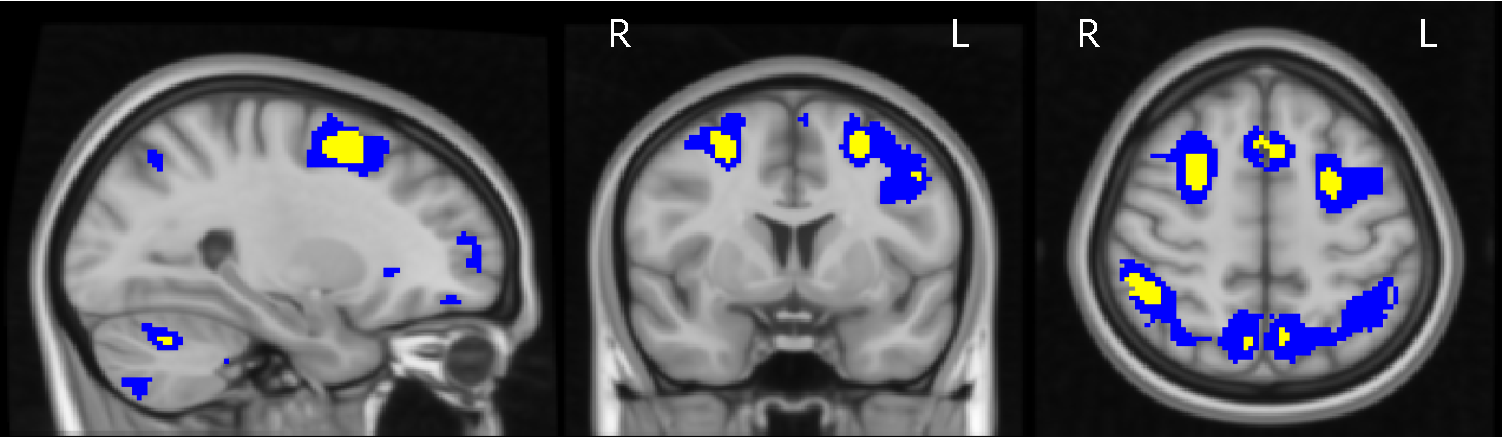
\includegraphics[height=45.5mm]{CIC_Fig1_Algorithm1_c12.pdf}\\
        \bottomrule
    \end{tabular}
\end{adjustbox}
    \captionof{figure}{Slices views of the Cohen's $d$ Confidence Sets obtained from applying Algorithm \ref{alg:one}.\ to the HCP working memory task data, using three Cohen's $d$ effect size thresholds, $c = 0.5, 0.8$ and $1.2$. Comparing with Fig.\ \ref{fig:HCP_Algorithm_3} and Fig.\ \ref{fig:HCP_Algorithm_2}, the CSs presented here are slightly more conservative than the corresponding CSs obtained with Algorithm \ref{alg:two}. and Algorithm \ref{alg:three}.\ (in the sense that the red upper CSs here are smaller, and blue lower CSs are larger). This is consistent with the simulation results obtained in Section \ref{sec:2D_sim_results} and \ref{sec:3d_sim_results}, where the empirical coverage for Algorithm \ref{alg:one}.\ was consistently larger than the other two methods.}
    \label{fig:HCP_Algorithm_1}
\end{table}

\begin{table}[!htbp]
\hspace*{-0.5cm}
\begin{adjustbox}{center}
\centering
    \begin{tabular}{cm{50mm}m{50mm}m{50mm}}
       \toprule
         Threshold $c$ & \hspace{1.4cm} Sagittal (X = 63) & \ \hspace{1.15cm} Coronal (Y = 130) & \hspace{1.0cm} Axial (Z = 124)\\
        \midrule
        0.5 Cohen's $d$ & 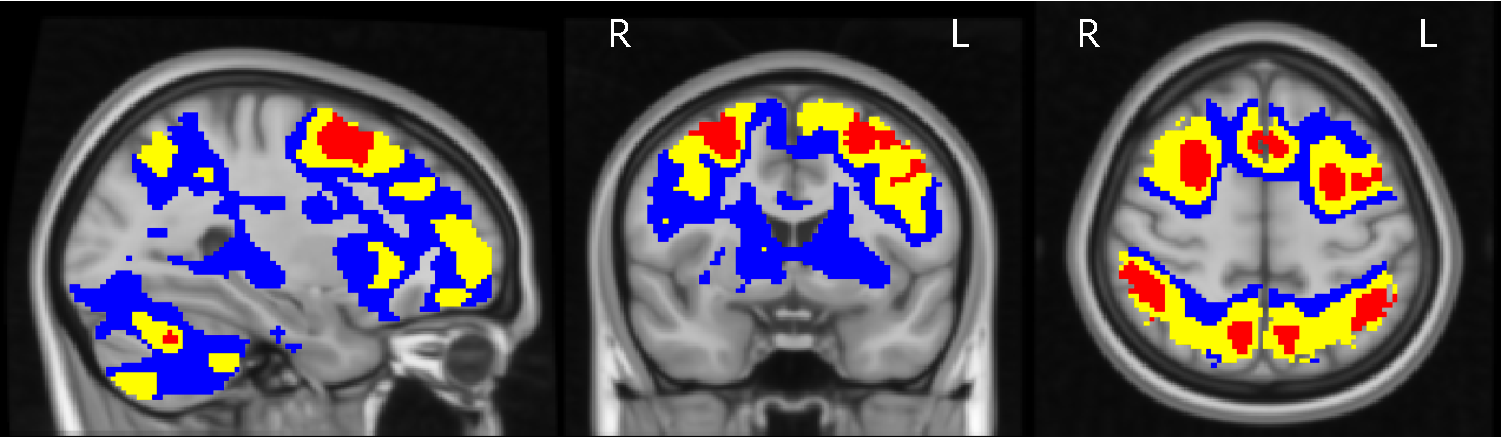
\includegraphics[height=45.5mm]{CIC_Fig1_Algorithm2_c05.pdf}\\
        0.8 Cohen's $d$ & 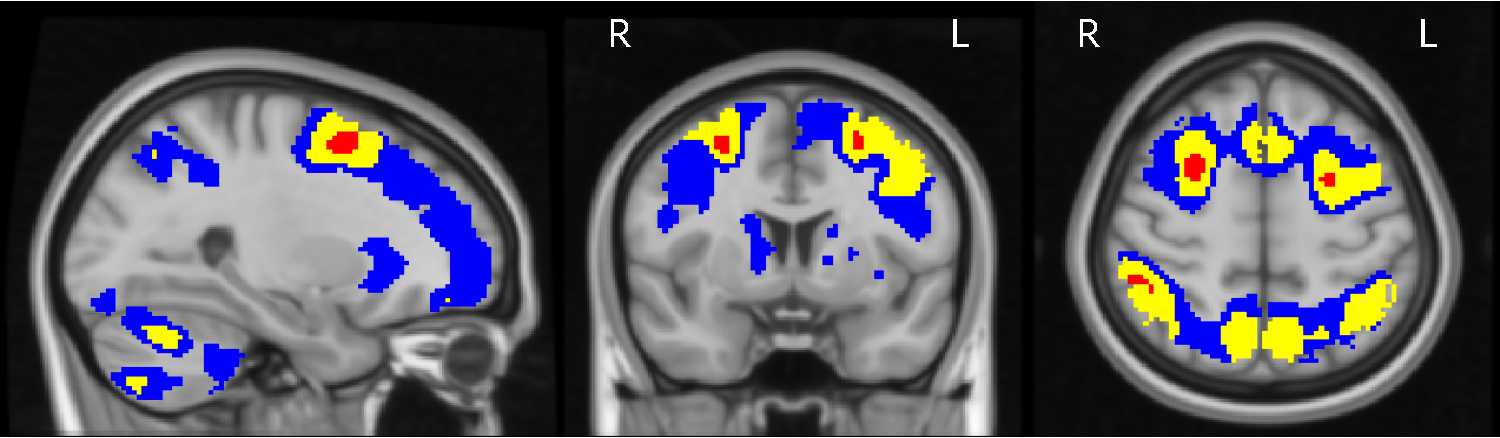
\includegraphics[height=45.5mm]{CIC_Fig1_Algorithm2_c08.pdf}\\
        1.2 Cohen's $d$ & 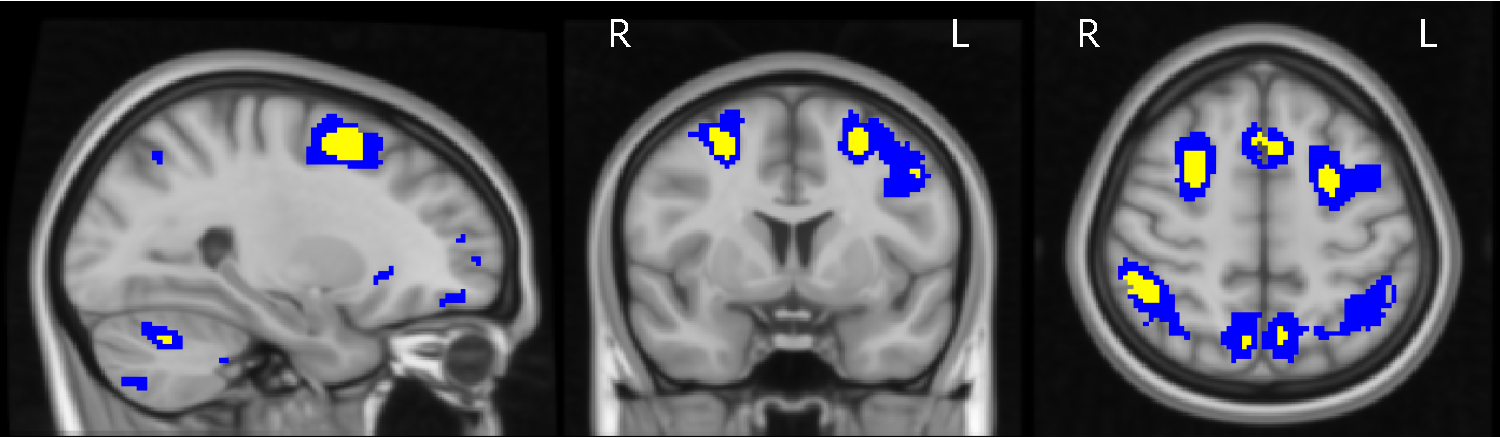
\includegraphics[height=45.5mm]{CIC_Fig1_Algorithm2_c12.pdf}\\
        \bottomrule
    \end{tabular}
\end{adjustbox}
    \captionof{figure}{Slices views of the Cohen's $d$ Confidence Sets obtained from applying Algorithm \ref{alg:two}.\ to the HCP working memory task data, using three Cohen's $d$ effect size thresholds, $c = 0.5, 0.8$ and $1.2$. Comparing with Fig.\ \ref{fig:HCP_Algorithm_3}, the upper and lower CSs presented here are almost identical to the corresponding CSs obtained with Algorithm \ref{alg:three}.}
    \label{fig:HCP_Algorithm_2}
\end{table}